%!TEX root = ../template.tex
%%%%%%%%%%%%%%%%%%%%%%%%%%%%%%%%%%%%%%%%%%%%%%%%%%%%%%%%%%%%%%%%%%%%
%% chapter4.tex
%% NOVA thesis document file
%%
%% Chapter with lots of dummy text
%%%%%%%%%%%%%%%%%%%%%%%%%%%%%%%%%%%%%%%%%%%%%%%%%%%%%%%%%%%%%%%%%%%%

\typeout{NT FILE chapter4.tex}

\chapter{Data Preprocessing}
\label{cha:data_preprocessing}
\hspace{10px}By definition, data preprocessing is the set of all data transformation, manipulation or dropping procedures before its use in supervised machine learning algorithms. In a real-world data science project, data preprocessing is one of the most important steps to be taken to ensure the success of a model, that is, between two models with the same data set the one that has undergone the proper data preprocessing procedures and feature engineering is what will have a more noticeable results. The figure below shows all the steps to be taken in the construction of a viable machine learning predictive algorithm, in it we can see that data preprocessing is an indispensable step before the application of any machine learning algorithm.

\begin{figure}[h]
    \centering
    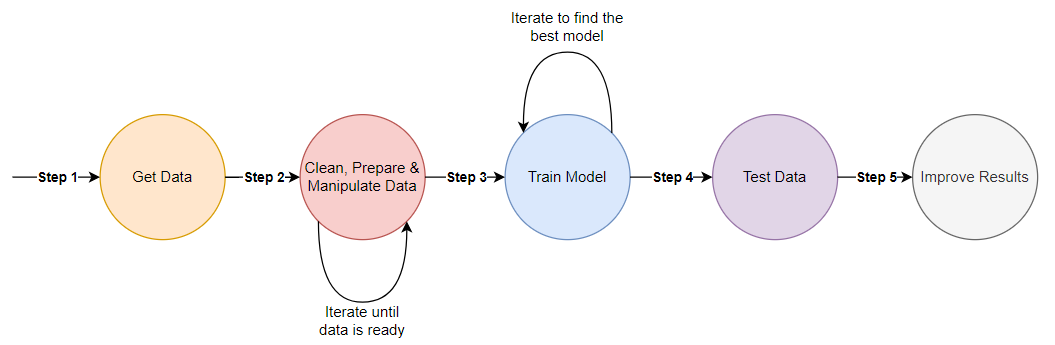
\includegraphics[width=0.9\textwidth,height=0.2\textheight]{Chapters/Figures/data preprocessing.png}
    \caption{The process of machine learning}
    \label{fig:preprocessing}
\end{figure}


The inability of machine learning and data mining algorithms to work with raw data further reinforces the need to apply transformations to the data to bring it into a more understandable formats. Also, in real-world data, data representation is often feature intensive and having irrelevant and redundant information or noisy and unreliable data makes knowledge discovery during the training phase much more difficult. Data preprocessing can also affect how the results of the final data processing can be interpreted. Which, in this case, can have a devastating consequence in the interpretation of the results and future diagnoses \cite{Paolo}. The main function of data preprocessing is to check the quality of the data before any analysis\cite{Pyle}, especially in computational biology. Such action is performed through 3 tasks: Data cleaning, Data editing and Data reduction. Within each task, there are several steps that will be covered later in this chapter and will be important for handling and cleaning the data set before applying feature selection and extraction algorithms, such as split data into training and test data sets, handling missing values and correlated features, taking care of categorical features etc.


\section{Missing data} % (fold)
\label{sec:missing_data}
\hspace{10px}Missing data is a daily problem that affects any data-related work and can show up in any type of data. By definition Missing data (or missing values) are data values that are not stored for a variable in the observation of interest, is common to find in almost all surveys and can have a significant effect on the tools that can be drawn from the data\cite{Graham}. These data types are defined as unavailable values and can be of any type, from missing string, incomplete resource, missing files, incomplete information, data entry error, etc. They can have different representations, from "?", or -999 and often by "n/a"\ or "null", in the image \ref{fig:dataset} it is possible to verify the existence of these same values with the representation of NaN in the features "GDC\_FILTER"\ and "COSMIC".

The absence of these values can cause several problems during and after the application of the algorithms. The absence of data reduces the statistical power of the probability of the test rejecting the null hypothesis when it is false. It can cause bias in the estimation of parameters and reduce the representativeness of the samples, i.e the sample loses relevance. All of this can complicate the analysis of the study and impair its validity, which ultimately leads to invalid conclusions.\cite{Hang} With the evolution and development of new algorithms and automatic learning packages, there are already some capable of detecting and automatically dealing with data absent. However, it does not remove the need to transform and analyze the missing data manually. Among the numerous strategies for dealing with missing data the two most common is to replace all missing values by a fixed value, for example zero, or by the average of all available values in the column. However, these approaches are not always the most correct, to know which is the most correct strategy to apply in our data set will depend on the domain and the type of missing data.


\subsection{Detecting Missing data and their type} % (fold)
\label{sec:document_structure}
\hspace{10px}According to Donal B. Rubin in \cite{Rubin} and in the book \cite{Berthold} missing data is divided into 3 types of missing data. This division is made by taking into account the mechanisms of missingness, the description of the different types is made below, going from the simplest to the most general.

\begin{itemize}
  \item \textbf{Missing completely at random (MACR):} It means that the probability of a value being absent does not depend on known values or the missing value itself, but on some other reason. The existence of missing data due to equipment failure or samples being lost or unsatisfactory, are examples of MCAR. The statistical advantage of these types of missing data is that the analysis remains impartial, that is, the estimated parameters are not influenced by the absence of data.
  
  \item \textbf{Missing at random (MAR):} Data is considered MAR when the probability of a missing instance may depend on other known values but not on the missing value itself. Research example: whether or not there is data referring to a feature, the lack of data does not depend on the feature itself, but may depend on values of another feature. Although randomness does not produce bias, MAR data cannot be ignored. If a missing variable is MAR, the possibility of there being a dropout of that variable in each case, is conditionally independent of the variable, being possible to predict the value through other variables observed.

  \item \textbf{Missing not at random (MNAR):} These are data whose characteristics do not correspond to those of MCAR or MAR, so they fall into the category of Missing not at random (MNAR). The probability that an instance is missing depends on the value of the variable itself. These type of data are very problematic since the missingness is specifically related to what is missing, the only way to get an unbiased estimate of the parameters is to model the missing data, which requires a greater understanding and domain knowledge of the lost variables.
 
\end{itemize}

After understanding the differences between MACR, MAR and MNAR we are able to classify the type of missing data for our dataset. The data dictates information, specific characteristics of each mutation based on a set of features, each variable within each feature is independent of each other, i.e, there is no relationship of variables within the same feature. The type of information contained in features varies between float, int64, bool and object, thanks to this variety of data types and a huge discrepancy in the number of NaN's in each feature (some with only 1 or 6 and others with 100\% or 80\% with ocupied with nan), the probability of a variable being dependent on another from a different feature is low. Nevertheless, since we are dealing with mutations from cancer cells, the fact that there is no information in a given feature may well be a consequence of the value (or what it represents) of another feature within the same mutation, for example, depending on the gene where the mutation was discovered, its representation in the data table may or may not have compromised values or have some data missing. Thus, the NaN are of the MAR type which means that some values can be predicted through other observed variables.

However, in all, there is still a large percentage of missing data, in a data set with 1,253,880 cells of information 40.86\% of this information is occupied with NaN values which does not bring any additional information to our problem. With \textit{X.info(verbose = True, show\_counts = True)} it is possible to analyze in detail the data type of each feature, the number of non-null cells within each feature, among other information relative to the data set. The figure \ref{fig:missing_values} represents, in a downward manner, the number of null cells corresponding to each feature after applying the following lines of code: \textit{m = X.isna().sum().tolist()} and \textit{m.sort(reverse =True)}. 

\begin{figure}[h]
    \centering
    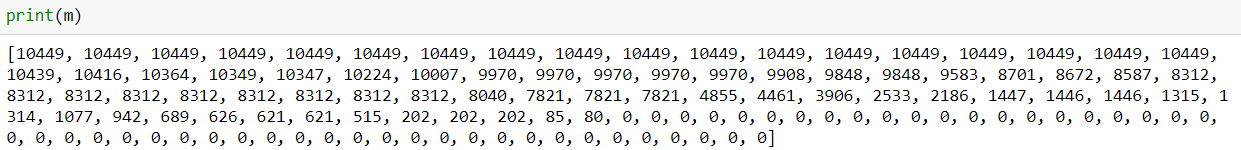
\includegraphics[width=0.9\textwidth,height=0.1\textheight]{Chapters/Figures/missing_values.png}
    \caption{List of missing data from a given data set}
    \label{fig:missing_values}
\end{figure}




\subsection{Handling Missing Values} % (fold)
\label{sec:handling_missing values}
\hspace{10px}By determining the list of missing data for a specific data set, it becomes easier to see the percentage of missing data corresponding to each feature. The code below represents the calculation of that same percentage, each value is stored in the list \textit{mising\_ratio} in the same position where it is entered in the original list. When analyzing the percentages of \textit{missing\_ratio} we see that there is a huge discrepancy in the missing values, there are features with 100\%, 90\%, 86\%, 37\%, 10\% and even with 0.8\% and 0.6\% of missing values. Of course, some of these characteristics will not contribute or almost nothing to the analysis of values, namely the characteristics with 100\% and 90\%, it is difficult to estimate the remaining values without having additional information, hence the need to deal with these features.
\begin{lstlisting}[language=Python]
    #percentage of missing data 
    missing_ratio = []
    for i in m:
        value = (i/len(X))*100
        missing_ratio.append(value)
    missing_ratio
\end{lstlisting}

Over the years, several methods have been presented to deal with missing values, these methods are separated into two main groups: deletion and imputation. Within the deletion group there are 3 most common methods: list-wise exclusion, pairwise exclusion and elimination (dropping) features. List-wise exclusion is the most used approach for dealing with missing data, it consists of omitting the cases where there is missing data and analyzing the remaining data. This approach, also known as complete-case analysis (CCA), only works if the sample is large enough and the missing data is of the MCAR type. Since our data is of the MAR type, this strategy is not recommended and a simple way to confirm this, by deleting all the lines where one or more values are missing, we quickly see that the data set is empty, because there is at least one missing value in each of the rows of the data set. As with list-wise exclusion, pairwise exclusion or available case analysis (ACA) is only recommended for missing data that are MCAR. In this case, only the missing observations will be ignored and the analysis is carried out on the remaining variables. Since pairwise exclusion uses all the observed information, it preserves more information than a list-wise. However, the analysis becomes deficient in the presence of too many missing observations and it becomes impossible to compare different analyzes (data sets) since only all available cases are considered. In the presence of too much missing data for a variable, a viable option would be to exclude the variable or column from the dataset given a certain threshold, eg 60\% or 90\%. This method is not advisable because a more adequate analysis of the data is necessary and there is some kind of improvement in the model's performance after the variable is excluded. However, for our problem at hand, this would be the most appropriate strategy. The presence of variables with 0\% information (100\% missing) can bring problems in future analysis, poor precision or false conclusions. The best way to deal with these variables would be to exclude all those that have all values with NaN,\ \textit{pandas.DataFrame.dropna} is the method used to remove all missing values by adding the parameters \textit{axis = 1}, \textit{how = all}, and \textit{inplace=True} it is possible to exclude the columns with NaN in all row values.

Unlike deletion approaches, the aim of imputation methods is to fill the missing values with a more reasonable values. The use of deletion approaches to discard samples (rows) or entire features (columns) causes loss of information, which is not always the intended solution, which makes imputation the most explored approach. Following the same structure, the imputation techniques are divided into two subgroups: single imputation and multiple imputation. In single imputation, only one imputation value is generated for each of the missing variables. One of the disadvantages of this strategy is that the generated value is treated as the true value, omitting the fact that the imputation method does not provide the exact value and so makes it ignore the uncertainty of missing values. Most simple imputation methods follow three main procedures: replacement using existing values, replacement using statistical values and replacement using represented values. The use of each of these procedures will depend on the type of values where they will be applied. Some only work on numeric values while others work with both numeric and nominal columns. Table \ref{table:1} bellow, succinctly shows the categorization of these strategies.

\begin{table}[h!]
\centering
\begin{center}
\begin{tabular}{ | m{5.5em} | m{5cm}| m{5cm} | } 
 \hline
 \textbf{Replacement using:} & \textbf{Only for numerical features} & \textbf{For both numerical and categorical features} \\ 
 \hline
 \textbf{Existing values} & maximum or minimum  & previous,  next or fixed value\\
 \hline
 \textbf{Statistical values} & mean, mode, median and average or linear interpolation & most frequent value\\
 \hline
  \textbf{Represented values} & regression algorithms & k-Nearest, regression and classification algorithms \\ 
 \hline
\end{tabular}
\caption{Characterization of Single imputation methods}
\label{table:1}
\end{center}
\end{table}

In multiple imputation, as the name implies, several/multiple imputed values are generated for each of the missing observations, meaning that several data sets with different imputation values are created. This is an imputation approach based on statistics and on the contrary of simple imputation methods, which have the disadvantage of not considering the uncertainty of the imputed values, which leads to the imputed values considered as real values, which in turn do not take into account the standard error causing bias in the results\cite{Azur}. Multiple imputation creates multiple "complete"\ data sets capable of filling in the missing values multiple times. The best known algorithm is Chained Equation Multiple Imputation (MICE). However, this strategy is not always the best, the fact that multiple datasets are created can lead to an increase in algorithm complexity and memory problems.

To make data analysis and processing easier, the chosen approach was to create functions that analyze sections of the data set. In this case, only columns with values of type float were chosen, since they have the largest number of NaN values, they require greater care and special attention. The \textit{handle\_nan\_values} function, shown below, represents the process of eliminating the columns that are below a given threshold and applying a imputation technique to fill the remaining NaN values present in the columns, with a \textit{mean} or \textit{most\_frequent} strategy depending on the type of data to be applied.

\begin{lstlisting}[language=Python]
def handle_nan_values(X):
    
    MC3_replace = {"Unknown": False,"False":False,"True":True}
    CAN_replace = {np.nan: "NO"}
    PICK_replace = {np.nan: 0.0}
    PHENO_replace = {np.nan: "trait","1":"disease","0":"phenotype"}
    MINI_replace = {np.nan:0}
    GENE_PHENO_replace = {np.nan:2}
    
    #Handle nullvalues in specific columns
    X["CANONICAL"] = X["CANONICAL"].replace(CAN_replace)
    X["PICK"] = X["PICK"].replace(PICK_replace)
    X["PHENO"] = np.where((X.PHENO == "1;0"), "NaN", X.PHENO)
    X["PHENO"] = X["PHENO"].replace(PHENO_replace)
    X["MINIMISED"] = X["MINIMISED"].replace(MINI_replace)
    X["GENE_PHENO"] = X["GENE_PHENO"].replace(GENE_PHENO_replace)
    
    #Handle mixed types in MC3_Overlap column
    if X["MC3_Overlap"].dtype == "object":
        X["MC3_Overlap"] = X["MC3_Overlap"].replace(MC3_replace)
    
    
    #Remove columns with all rows values as null
    X.dropna(axis=1,how="all", inplace = True)
    
    #Remove columns that are below treshold 0.70(70%)
    length = len(Y)
    thresh = length*0.70
    X.dropna(axis=1,thresh=int(thresh), inplace = True)
         
    #Fill remaining null values
    cateogry_columns = X.select_dtypes("object").columns
    for column in X.columns:
        if X[column].isnull().any():
            if(column in cateogry_columns):
                X[column] = X[column].fillna("NaN")
            else:
                X[column] = X[column].fillna(0)
    return X
\end{lstlisting}
\hspace{10px} As a first step, the columns that have all their values as NaN are removed, as they do not contribute any additional information, are considered as noisy data or meaningless data, which are not able to be read or used by the programs and algorithms. Then, we proceeded to the selection of a limit for the minimum number of useful information contained in each column. The threshold chosen was 70\%, that is, only columns that contain at least 70\% of information are preserved (this calculation is done by the number of lines of each data set, for example, 10449 lines then the threshold would be 10449*0.7), the choice of this value is due to the fact that most of these columns contain little or no information, for example of the 21 columns with float values only 1 contains 90\% of information and only 2 are above 70\% as the remainder fall in the range of 10\% or less making it almost impossible to accurately predict the remaining missing values. 

The calculation of the NaN values for columns of types different than type object was done through the use of a imputation technique. From \textit{sklearn.impute} we use the SimpleImputer with a strategy of \textit{mean} which replaces the missing values using the mean along each column. This has the benefit of not changing the sample mean for each column. After that, all that remains is to deal with the NaN values in the object type columns.

Initially the replacement was done through existing values using the \textit{pad} method also known as forward replacement, where the last valid observation is used as the replacement value, until reaching the next valid value within each column. However, this method as well as ffill method only do forward value replacement starting at the first valid value (other than NaN) and if there is any NaN value at the beginning of the column these are ignored by the method and remain untreated, the same applies to bfill or backfill that propagate the valid values backwards. Another problem with these methods is that in the presence of a feature with only one valid value, all other values would be replaced by this one, making this feature biased, thus manipulating the result into favoring this feature. And depending on the position of the first valid value, these methods may or may not work. Therefore, the best solution was to apply the same imputation technique used for the other value types, only this time with the \textit{most\_frequent} strategy as strategy \textit{mean} or \textit{median} don't work with object type values.

\section{Correlated Features}
\label{sec:correlated_features}
\hspace{10px}As the number of NaN values, up to this point, is non-existent, the next step is to check the existence of correlated features if so the best solution is to drop them. By definition, correlation means a mutual relationship between two or more things, it is a statistical expression that concerns how close two variables are to having a linear relationship with each other\cite{Vishal}. The purpose of the correlation is to see if the values from two features, whether are small or large, are paired with each other. In statistics, this is measured by an adjustment function called the correlation coefficient \cite{corrwebsite}. This coefficient varies between -1 and 1, if is between [0,1] then the values are positively correlated, otherwise they are negatively correlated.

In regression, the main focus is trying to predict dependent values through one or more independent values. To know how well a regression model fits the data, determining the model's variance is the best choice and by the assumption that the dependent variable is normally distributed with variance \(\sigma^2\), then we can say that \(\sigma^2 = (X^TX)^{-1}\). For the model to be stable, the value of \(\sigma^2\) mus be low. If \(\sigma^2\) is high means the model is very sensitive to the data and might not perform well. With the existence of highly correlated features within our data set makes the variance of the weight vector of the regression model be large. So, when two features have high correlation, the best solution is to drop one of the two features.

A piece of code extracted from \href{https://chrisalbon.com/code/machine_learning/feature_selection/drop_highly_correlated_features/}{Chris Albon’s} work is provided below. In it, the correlation matrix is created to later find the features that have correlation greater than 95\%.

\begin{lstlisting}[language=Python]
def get_correlated_cols(X):

    # Create correlation matrix
    corr_matrix = X.corr().abs()

    # Select upper triangle of correlation matrix
    upper = corr_matrix.where(np.triu(np.ones(corr_matrix.shape),
            k=1).astype(bool))
           
           
    # Find index of feature columns with correlation greater than 0.95
    for column in upper.columns:
        if any(upper[column] > 0.95):
            to_drop = [column]
    return to_drop
\end{lstlisting}


\section{Duplicated Columns and Similar Value Columns}
\label{sec:duplicated_similar_columns}
\hspace{10px}Once the columns with high correlation are already eliminated, we move on to the removal of duplicate columns and columns with similar values. In the context of data quality, the removal of duplicates consists of identifying and then removing instances where there is more than one record of the same instance.

Data are collected from several clinical and genomic cancer studies. As researchers update studies or make new discoveries, they often enter their data more than once. This, in turn, leads to data sets having more than one equal feature, possibly with conflicting information.

Identifying and removing or merging these duplicate data set features will create a full version of the truth about the data set, save time and resources by not running identical data multiple times during feature selection or extraction algorithms and the data set becomes more accurate, as no information is lost when removing duplicate features.

\begin{lstlisting}[language=Python]
def get_duplicated_value_cols(X):
    
    count = 0
    deleted = 0
    columns_not_accepted = {"Exon_Number","Transcript_ID",
                            "Allele","Reference_Allele"}
    
    #get matrix of duplicated columns
    duplicated_columns = X.T[X.T.duplicated(keep=False)].T.columns
    print(duplicated_columns)
    
    #remove duplicated columns
    for col in duplicated_columns:
        #if col in columns_not_accepted: 
        X.drop(col,axis=1, inplace = True)
        deleted += 1
        count += 1
        
    print("Columns with duplicated values:", count)
    print("Columns deleted:", deleted)
    return X
\end{lstlisting}

With the help of the python framework it is possible to create a matrix that identifies the duplicated columns, this matrix is implemented in the \textit{get\_duplicated\_value\_cols} function represented above, followed by an iteration to select the columns to be removed. According to the "GDC Data User's Guide"\ the EXON, Feature and Reference\_Allele columns are already represented in the data set but with a different name, that is, taking into account the characteristics of each column and what each one represents these were the columns chosen to be removed.

Now, finally, it is necessary to find the features where the majority share of the values are akin. The principle is the same as duplicated columns, therefore these features will not help us to differentiate between driver mutations and so features where more than 90\% of the values are similar have been removed from the data set.

\begin{lstlisting}[language=Python]
def get_similar_value_cols(X):
    thresh = 90
    number_of_cols = 0
    similar_values = []
       
    for c in X.columns:
        #percentage of each value inside columns
        percent_vals = (X[c].value_counts()/len(X)*100).values
        
        #filter columns where more than 90% values are same
        if percent_vals[0] >= thresh:
            similar_values.append(c)
            number_of_cols += 1 
            
  return similar_values
\end{lstlisting}

\section{Outliers} % (fold)
\label{sec:outliners}
\hspace{10px} As stated in \cite{Kuhn} outliers are samples that are exceptionally far from the mainstream of the data. With this definition, it is possible to say that an outlier is an observation highly different from the rest. These observations can distort the distribution of our data and parameters like means, standard deviations, and correlations. Hence, it is important to deal with them while preparing our data before further analysis.

However, it is very difficult to define and identify outliers in general because of the specifics of the data set. It is mandatory to first analyze the observations before deciding whether a given value is an outlier or not. Dropping outliers can be very dangerous and only done under specific conditions, such as, when we know in advance that the outlier is completely wrong (eg. knowing the range our data falls in and remove outliers outside that range), working with large data, the sample won’t be hurt by dropping questionable outliers and if the outlier does not change the results but does affect assumptions. 

Since our results are critical, identify which mutation is a driver mutation, even the smallest of changes in the data set will make a difference. Sometimes these changes can be legitimate observations and the reason why this specific mutation was selected as a driver mutation. Another reason not to remove outliers is if there is a large number of outliers in the data set. Outliers are rare, so if a data set has, lets say, 20\% are outliers means that there's something of interest within the data set that requires further analysis. One way to check this is to perform the \textbf{Z-Score} test where the z value is between -3 and 3 and all values that fall outside this range are considered outliers. After performing this test the result was 2046 values considered as outliers
which corresponds to 20\% of our data set. 

In this situation, it is not recommended to discard outliers but nevertheless the analysis should be run both with and without them. This time the analysis of the algorithms will be perform only with the outliers.

\section{Categorical Features} % (fold)
\label{sec:categorical_values}
\hspace{10px}The next step will be to deal with categorical features. As machine learning models use mathematical equations categorical data are not accepted, therefore, it is necessary to convert them to integers. There are currently only 2 ways to do this, using the Label Encoding or One Hot Encoding method. The big difference between the two methods is that unlike One Hot Encoding which creates a column for each categorical value and this column has a value of 1 if this value exists in the initial data otherwise it will be 0, in Label Encoder the categorical values themselves are converted to numeric labels.
The lack of creating additional columns makes Label Encoding the ideal method to apply in our data set. The creation of new columns only leads to an exponential increase in the size of the data set from 9.5MB to more than 2.5GB of information which makes the application of feature extraction and selection algorithms costly on a temporal and spatial level.

\begin{lstlisting}[language=Python]
#Handling categorical values
def handle_categ_values(X):
    labelencoder_x = LabelEncoder()
    
    #Execute LabelEncoder for each categorical column
    for n in X.columns:
        X[n] = labelencoder_x.fit_transform(X[n])
    return X
        
 #Handling categorical values for variable Y
 labelencoder_y= LabelEncoder()  
 Y = labelencoder_y.fit_transform(Y)
\end{lstlisting}

The code above describes the application of the Label Encoder method for the X and Y variables mentioned above. Here, a \textit{LabelEncoder} object is instantiated, the \textit{fit\_transform} method makes the \textit{LabelEncoder} fit the desired column and proceeds with its transformation and application, it is the simplified way to apply first the \textit{fit} method and then the \textit{transform} method. Applying the \textit{info} method to both X and Y shows us that the categorical values, in this case object and boolean, have all been converted to integer values and are ready for the next step of data preprocessing. To ensure that all data in X are of the same type, method \textit{fit\_transform} is applied to all columns of the data set.

\section{Train-Test Split} % (fold)
\label{sec:test_train_split}
\hspace{10px}Although the procedure of separating data into train data and test data is one of the most important steps in machine learning, to fulfill our goal, this step will only be applied after using feature selection and extraction algorithms. These algorithms can only be applied to the original data set and before any separation of the data into testing data and training data, if this does not happen, null values will reappear and it becomes more difficult to treat them in the middle of the algorithm implementation. The train-test split procedure is mainly used to estimate the performance of machine learning algorithms when they are used to create results on unused data to train the model. It's a quick and easy-to-run procedure, whose results allows you to compare the performance of machine learning algorithms for predictive modeling problems.

Train-test, as the name implies, is to convert or split the original data set into 2 subsets the test and the training, where the training data set is used to fit the machine learning model and the test data set is used to later evaluate this same model.

The scikit-learn library has a innate function named \textit{train\_test\_split}. For this function, X and Y will be passed-in as arguments which splits X and Y with a, let's say 30\% for the \textit{test\_size} leaving 70\% for the \textit{train\_size}, successfully splitting between x\_train, x\_test, y\_train, and y\_test with a \textit{random\_state} of 42.


\section{Features Scaling} % (fold)
\label{sec:feature_scaling}
\hspace{10px} This is the last step of data preprocessing, which is scaling and normalization of the data set. The purpose of data scaling data is transforming the data so that it fits within a specific scale. On the other hand, normalization is to change the data so it can be described as a normal distribution. Normalization will only be used prior to machine learning techniques that assumes the data is normally distributed such as LDA, ANOVA and t-test.

It has been proven by testings that the Machine Learning and Deep Learning algorithms perform better with a normalized and scaled data set than with a non-normalized ans non-scaled data set. StandardScaler and Normalization are the 2 possible ways to normalize the data. Both StandardScaler and Normalization are very similar, however StandardScaler is simpler to apply than Normalization.

By importing StandardScaler from the  sklearn.preprocessing libary, similar to LabelEncoding method, only this time the StandardScaler.fit\_transform will be apply on our X data set. After applying all the data preprocessing steps, the data set will be similar to Figure \ref{fig:xtrain_data} and ready to be used in the algorithms described in the following chapters.


\begin{figure}[h]
    \centering
    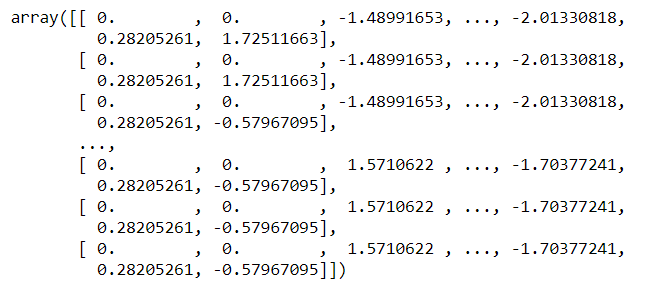
\includegraphics[width=0.7\textwidth,height=0.17\textheight]{Chapters/Figures/standardScaler.png}
    \caption{Normalized X data}
    \label{fig:xtrain_data}
\end{figure}